\subsection{Quick Sort}

\subsubsection{Ý tưởng}

Quick Sort cũng là một thuật toán sắp xếp dựa trên phương pháp "chia để trị", nhưng cách thức chia và hợp nhất khác so với Merge Sort.
% \begin{itemize}
%     \item Chọn pivot: Đầu tiên, một phần tử trong mảng được chọn làm pivot.
%     \item Phân hoạch: Mảng được chia thành hai phần con:
%     \begin{itemize}
%         \item Các phần tử nhỏ hơn pivot.
%         \item Các phần tử lớn hơn hoặc bằng pivot.
%     \end{itemize}
    
%     \item Đệ quy: Quá trình trên được lặp lại đệ quy cho mỗi phần con cho đến khi mảng con chỉ còn một phần tử hoặc không còn phần tử nào.
% \end{itemize}

Thuật toán quicksort cổ điển để sắp xếp một mảng $A$ bao gồm bốn bước đơn giản sau:

1. Nếu số lượng phần tử trong $A$ là 0 hoặc 1, thì trả về.

2. Chọn bất kỳ phần tử $v$ nào trong $A$. Đây được gọi là phần tử trục (pivot).

3. Phân chia $A - \{v\}$ (các phần tử còn lại trong $A$) thành hai nhóm rời nhau: 
\begin{itemize}
    \item $A_1 = \{x \in A - \{v\} \mid x \leq v\}$
    \item $A_2 = \{x \in A - \{v\} \mid x \geq v\}$.
\end{itemize}

4. Trả về \{ \{$quicksort(A_1)$\}, $v$, \{$quicksort(A_2)$\} \}.

    
    
\subsubsection{Các bước hoạt động}
Xét mảng A như sau: 
\begin{center}
   A = \{5, 3, 8, 4, 6, 3, 2\} 
\end{center} 

Bước 1: Chọn phần tử chốt (pivot) là phần tử chính giữa của mảng là:
\[
\text{Pivot} = 4
\]

Bước 2: Di chuyển các phần tử nhỏ hơn hoặc bằng pivot về bên trái và phần tử lớn hơn về bên phải:
\[
\{3, 3, 2, 4, 5, 8, 6\}
\]

Bước 3: Gọi đệ quy, thực hiện đệ quy Quick Sort trên hai mảng con:
\begin{itemize}
    \item Mảng con bên trái: \(\{3, 3, 2\}\)
    \item Mảng con bên phải: \(\{5, 8, 6\}\)
\end{itemize}

Sắp xếp mảng con bên trái \(\{3, 3, 2\}\):
\begin{itemize}
    \item Chọn pivot: \(3\) (phần tử giữa của mảng con).
    \item Phân hoạch: \(\{2, 3, 3\}\).
    \item Kết quả: \(\{2, 3, 3\}\) (không cần đệ quy thêm).
\end{itemize}

Sắp xếp mảng con bên phải \(\{5, 8, 6\}\):
\begin{itemize}
    \item Chọn pivot: \(8\) (phần tử giữa của mảng con).
    \item Phân hoạch: \(\{5, 6, 8\}\).
    \item Kết quả: \(\{5, 6, 8\}\) (không cần đệ quy thêm).
\end{itemize}

Kết hợp mảng đã sắp xếp
Ghép các mảng con lại:
\[
A = \{2, 3, 3, 4, 5, 6, 8\}
\]

\begin{figure}[H]
    \centering
    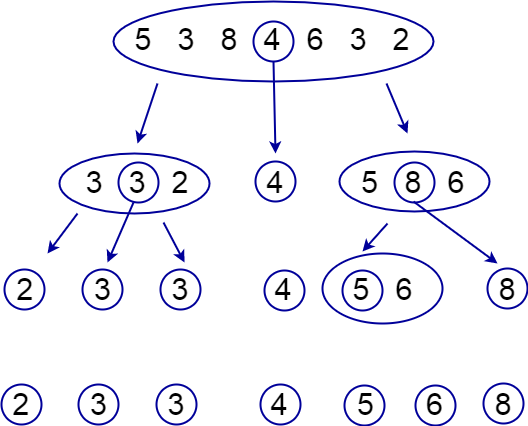
\includegraphics[width=0.8\textwidth]{img/quick_sort.png}
    \caption{\href{https://qnaplus.com/wp-content/uploads/2017/05/quick_sort.png}{Quick Sort Algorithm Diagram}}
\end{figure}

\subsubsection{Mã giả}
 
\begin{algorithm}[H]
\caption{Quick Sort}
\label{alg:quick-sort}
\begin{algorithmic}

\Require $A$ is an array of size $n$

\Function {partition}{\textit{A}, \textit{low}, \textit{high}}
\State $pivot \gets A[high]$
\State $i \gets low - 1$
\For{$j = low$ to $high-1$}
    \If{$A[j] < pivot$}
        \State $i \gets i + 1$
        \State Swap $A[i]$ and $A[j]$
    \EndIf
\EndFor
\State Swap $A[i+1]$ and $A[high]$
\State \Return $i+1$
\EndFunction

\Function {quick-sort}{\textit{A}, \textit{low}, \textit{high}}
\If{$low < high$}
    \State $pivot \gets$ \Call{partition}{A, low, high} \State
    \Call{quick-sort}{A, low, pivot-1} \Comment{Sort the left subarray}
    \State \Call{quick-sort}{A, pivot+1, high} \Comment{Sort the right subarray}
\EndIf
\EndFunction

\end{algorithmic}
\end{algorithm}


\subsubsection{Độ phức tạp}
\textbf{Độ phức tạp thời gian}

\footnote{Mục 7.7.5 \cite{dsa-analysis-cpp}}Giả sử một pivot ngẫu nhiên và $T(0) = T(1) = 1$. Thời gian chạy của quicksort bằng thời gian chạy của hai lệnh gọi đệ quy cộng với thời gian tuyến tính dành cho phân vùng (lựa chọn pivot chỉ mất thời gian không đổi). Điều này đưa ra mối quan hệ quicksort cơ bản 

\begin{equation}
T(n) = T(i) + T(n - i - 1) + cn \tag{2.8.1} 
\end{equation}

trong đó i là số phần tử của $A_1$. Xét ba trường hợp sau:

\subparagraph{1. Trường hợp xấu nhất}

Pivot là phần tử nhỏ nhất, mọi lúc. Khi đó i = 0, và nếu bỏ qua $ T(0) = 1$, là không đáng kể, thì hệ thức đệ quy là 
$$T(n) = T(n - 1) + cn,  n > 1$$ 								 
Sử dụng phương trình trên nhiều lần. Ta có:
\begin{align*}
T(n - 1) &= T(n - 2) + c(n - 1) \\
T(n - 2) &= T(n - 3) + c(n - 2) \\
\dots \\
T(2) &= T(1) + 2c   
\end{align*}
	 
Cộng tất cả các phương trình này lại, ta được 
$$T(n) = T(1) + c \sum_{i = 2}^{n}i = 1 + c \frac{(n - 1)(n + 2)}{2}$$

Để thấy rằng đây là trường hợp tệ nhất có thể, hãy lưu ý rằng tổng chi phí của tất cả các phân vùng trong các lệnh gọi đệ quy ở độ sâu d phải tối đa là $n$. Vì độ sâu đệ quy tối đa là $n$, điều này đưa ra giới hạn trường hợp tệ nhất là $O(n^2)$ cho Quick Sort.

\subparagraph{2. Trường hợp tốt nhất}

Trong trường hợp tốt nhất, pivot nằm ở giữa. Để đơn giản hóa phép toán, giả sử rằng hai mảng con đều có kích thước bằng đúng một nửa kích thước của mảng ban đầu.

$$T(n) = 2T(n / 2) + cn$$

Chia cả hai vế của phương trình trên cho n. 

$$\frac{T(n)}{n} = \frac{T(n / 2)}{n / 2} + c$$

Tương tự, ta được:
\begin{align*}
    \frac{T(n/2)}{n/2} &= \frac{T(n / 4)}{n / 4} + c \\
    \frac{T(n/4)}{n/4} &= \frac{T(n / 8)}{n / 8} + c \\
    \dots \\
    \frac{T(2)}{2} &= \frac{T(1)}{1} + c
\end{align*}

Chúng ta cộng tất cả các phương trình trên lại và lưu ý rằng có $\log{n}$ phương trình:
\begin{align*}
    \frac{T(n)}{n} &= \frac{T(1)}{1} + c \log{n} \\
    \implies T(n) &= n + cn\log{n} 
\end{align*}

Do đó giới hạn trường hợp tốt nhất là $O(n\log{n})$ cho Quick Sort.

\subparagraph{3. Trường hợp trung bình}

Giả sử rằng mỗi kích thước cho $A_1$ có khả năng xảy ra như nhau và do đó có xác suất là $\frac{1}{n}$. Giả sử này chỉ hợp lệ đối với cách chọn pivot và phân hoạch như trên. 

Với giả định này, giá trị trung bình của $T(i)$, và do đó là $T(n - i - 1)$, là $\frac{1}{n} \sum_{j = 0}^{n - 1}T(j)$. Phương trình  (2.8.1) trở thành: 

\begin{align*}
    & T(n) = \frac{2}{n} \left[\sum_{j = 0}^{n - 1}T(j) \right] + cn \\
    \implies  &nT(n) = 2 \left[\sum_{j = 0}^{n - 1}T(j) \right] + cn^2 \tag{2.8.2} \\
    \implies  &(n - 1)T(n - 1) = 2 \left[\sum_{j = 0}^{n - 2}T(j) \right] + c(n - 1)^2 \tag{2.8.3}
\end{align*}

Lấy phương trình (2.8.2) - (2.8.3), ta được:

$$nT(n)-(n-1)T(n-1)=2T(n-1)+2cn-c $$
Sắp xếp lại các số hạng và bỏ $-c$ không đáng kể ở bên phải, thu được: 

\begin{align*}
    nT(n)=(n+1)T(n-1)+2cn \tag{2.8.4}
\end{align*}

Bây giờ ta có một công thức cho $T(n)$ chỉ theo $T(n - 1)$. Chia phương trình (2.8.4) cho $n(n + 1)$: 

\begin{align*}
&\frac{T(n)}{n+1}=\frac{T(n-1)}{n}+\frac{2c}{n+1} \\
\implies &\frac{T(n-1)}{n}=\frac{T(n-2)}{n-1}+\frac{2c}{n} \\
\implies &\frac{T(n-2)}{n-1}=\frac{T(n-3)}{n-2}+\frac{2c}{n-1} \\
&\dots \\
\implies &\frac{T(2)}{3}=\frac{T(1)}{2}+\frac{2c}{3} \\
\end{align*}

Cộng các phương trình lại, cho kết quả:
\begin{align*}
&\frac{T(n)}{n+1}=\frac{T(1)}{2}+2c\sum_{i=3}^{n+1}\frac{1}{i} \tag{7.23} \\
\end{align*}

Tổng xấp xỉ $\ln(n + 1) + \gamma - 3/2$ , trong đó $\gamma \approx 0,577$ được gọi là hằng số Euler, do đó 

\begin{align*}
    &\frac{T(n)}{n+1}=O(\log n) \\
    \implies &T(n)=O(n \log n) 
\end{align*}


Kết luận về độ phức tạp thời gian:

 \begin{itemize}
    \item Trường hợp tốt nhất: $\Omega(n\log{n})$ 
    \item Trường hợp xấu nhất: $O(n^2)$
    \item Trường hợp trung bình: $\Theta(n\log{n})$
\end{itemize}


\textbf{Độ phức tạp không gian}

Quick Sort sử dụng số lượng hằng số các biến trung gian trong quá trình hoán đổi các phần tử lúc phân hoạch mảng, do đó độ phức tạp không gian là $O(1)$.


\subsubsection{Nhận xét}

Quick Sort và Merge Sort là hai thuật toán sắp xếp nổi tiếng dựa trên phương pháp chia để trị. Quick Sort thường được đánh giá cao về tốc độ thực thi nhờ việc không sử dụng mảng phụ và cấu trúc đơn giản. Tuy nhiên, hiệu suất của Quick Sort phụ thuộc rất lớn vào việc lựa chọn pivot. Nếu không may chọn phải pivot không phù hợp, thuật toán có thể rơi vào trường hợp xấu nhất với độ phức tạp $O(n^2)$. Ngược lại, Merge Sort luôn đảm bảo độ phức tạp $O(n \log{n})$ trong mọi trường hợp, nhưng thường tiêu tốn nhiều không gian bộ nhớ hơn do cần sử dụng mảng phụ. 

Trong thực tế, Quick Sort được sử dụng rộng rãi trong các thư viện sắp xếp của nhiều ngôn ngữ lập trình nhờ tốc độ nhanh và tính linh hoạt. Tuy nhiên, khi yêu cầu độ ổn định cao hoặc cần xử lý các tập dữ liệu lớn, Merge Sort vẫn là một lựa chọn đáng cân nhắc.

\textbf{Cải tiến}

Để khắc phục hạn chế về việc chọn pivot của Quick Sort, nhiều phương pháp cải tiến đã được đề xuất như chọn pivot ngẫu nhiên, median-in-medians, . Ngoài ra, các biến thể của Quick Sort giúp cải thiện hiệu suất trong các trường hợp cụ thể như Quick Sort ba đường phân hoạch (chia mảng thành 3 phần), Introsort (một thuật toán sắp xếp hybrid, kết hợp ưu điểm của cả Quick Sort và Heap Sort để đạt được hiệu suất cao trong hầu hết các trường hợp).

